\documentclass[../notes.tex]{subfiles}

\pagestyle{main}
\renewcommand{\chaptermark}[1]{\markboth{\chaptername\ \thechapter\ (#1)}{}}
\setcounter{chapter}{6}

\begin{document}




\chapter{Electronic Relaxation}
\section{Office Hours (Moe)}
\begin{itemize}
    \item \marginnote{2/13:}Use chemical shift as your $x$-axis in NMR plots.
    \item Hexylamine is our substance.
    \item Interpreting NMR data files: Column E is chemical shift; column C is peak intensity. Column D is hertz (not chemical shift).
    \begin{itemize}
        \item Chemical shift is in the rightmost column.
    \end{itemize}
    \item Fitting tutorial: If solver still isn't helping (you get an error message and no convergence), divide the absolute intensities by a million. You can also do this from the get-go.
    \item $M_z$ should be calculated for each carbon; it is the absolute integral value in the all-integrals spreadsheet.
    \item Don't let the peaks overlap in the plot of multiple vertically offset $T_1$ values.
    \begin{itemize}
        \item Use 3 plots.
    \end{itemize}
    \item R outputs standard error values automatically.
    \begin{itemize}
        \item In Excel, it's much more difficult.
        \item A residuals plot is a good thing to include, but there won't be points for it. Standard error also isn't worth points. Sarah will have them upload the rubric. Sarah opened the door to email her.
        \item We need standard error for all 6 regressions.
    \end{itemize}
    \item Sarah will send a source for literature values.
\end{itemize}



\section{Lecture 12: Electronic Relaxation and Fluorescence Spectroscopy}
\begin{itemize}
    \item \marginnote{2/14:}Today: What happens after absorption (fluorescence and relaxation).
    \item Motivating question: What is the fate of electronic excitations?
    \begin{itemize}
        \item Absorption to an electronic excited state takes a lot of energy.
        \item This energy needs to be dissipated to return to equilibrium via
        \begin{equation*}
            \ce{A^* -> A + energy}
        \end{equation*}
        \item Many possible routes (radiative [releasing low-energy photons] and non-radiative [various]).
    \end{itemize}
    \item Review: Electronic absorption leads to vibrational excitation which relaxes vibrationally.
    \begin{figure}[H]
        \centering
        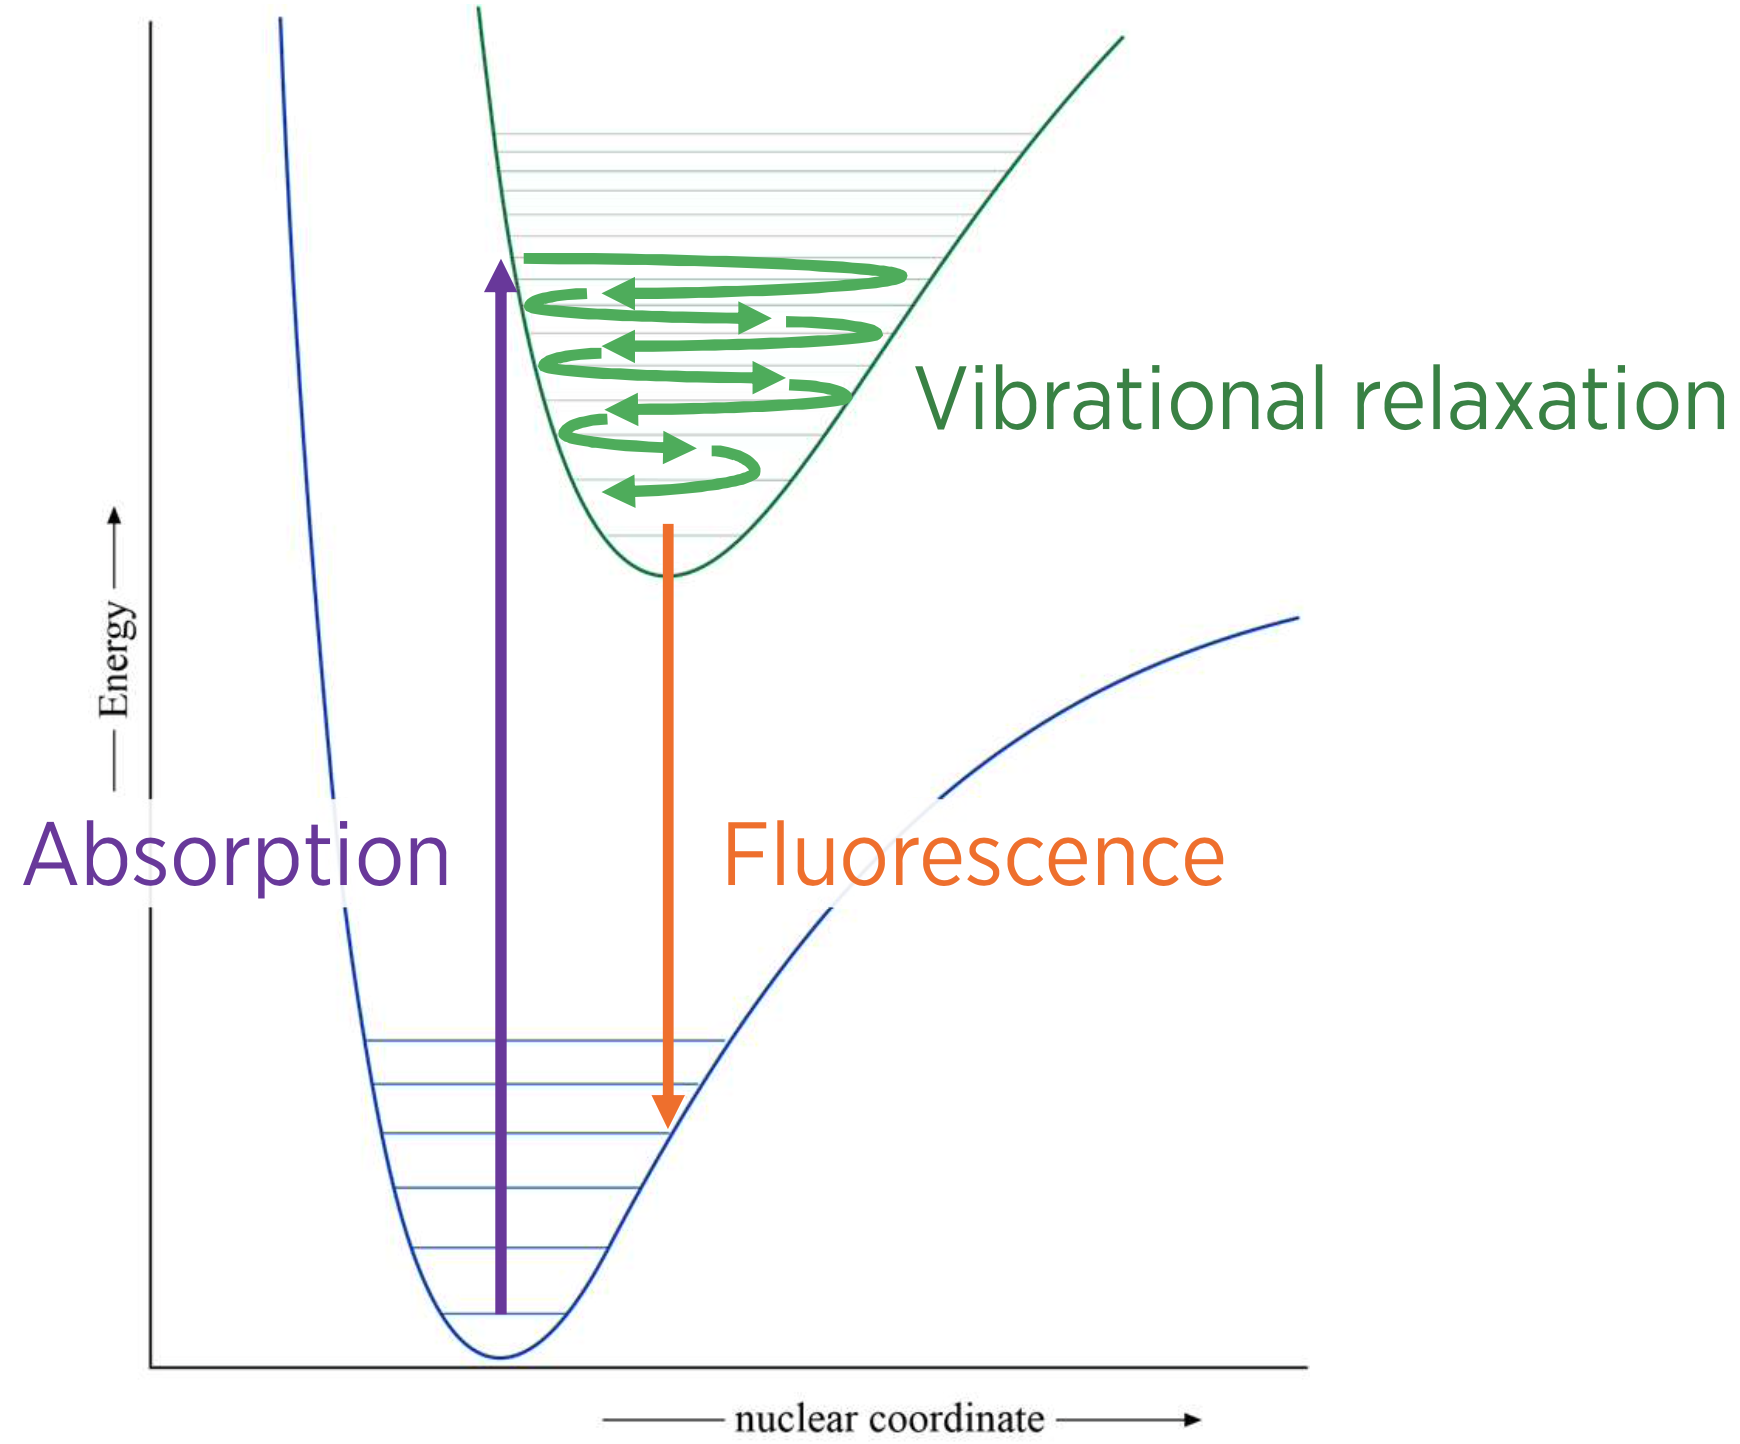
\includegraphics[width=0.4\linewidth]{excitationSteps.png}
        \caption{The photophysical excitation process.}
        \label{fig:excitationSteps}
    \end{figure}
    \begin{itemize}
        \item Vibrational energy dissipates non-radiatively via intramolecular vibrational energy redistribution and intermolecular collisions.
        \begin{itemize}
            \item No change in electronic state is involved.
        \end{itemize}
        \item The radiative path (fluorescence) is slower.
        \begin{itemize}
            \item $k_\text{rad}\ll k_\text{IVR}$.
            \item Most fluorescence occurs from $v'=0$. Further relaxation requires a change of electronic state.
        \end{itemize}
        \item Time scale of relevant processes.
        \begin{itemize}
            \item The vibrational period of a molecule is \SIrange{10}{100}{\femto\second}.
            \item Vibrational relaxation in solution takes \SIrange{1}{10}{\pico\second}.
            \item Fluorescence emission takes \SIrange{1}{10}{\nano\second}.
        \end{itemize}
        \item Once you get into the ground state, you have further vibrational relaxation.
    \end{itemize}
    \item $\bm{k_\textbf{rad}}$: The radiative fluorescence emission rate.
    \item $\bm{k_\textbf{nr}}$: The rate of all nonradiative processes leaving the flourescent state. \emph{Given by}
    \begin{equation*}
        k_\text{nr} = \sum_ik_{\text{nr},i}
    \end{equation*}
    \item $\bm{k_\textbf{IVR}}$: The \underline{i}ntramolecular \underline{v}ibrational \underline{r}elaxation rate.
    \item \textbf{Reorganization energy}: The amount of energy dissipated on one of the potential energy surfaces. \emph{Denoted by} $\lambda$.
    \begin{figure}[H]
        \centering
        \begin{subfigure}[b]{0.35\linewidth}
            \centering
            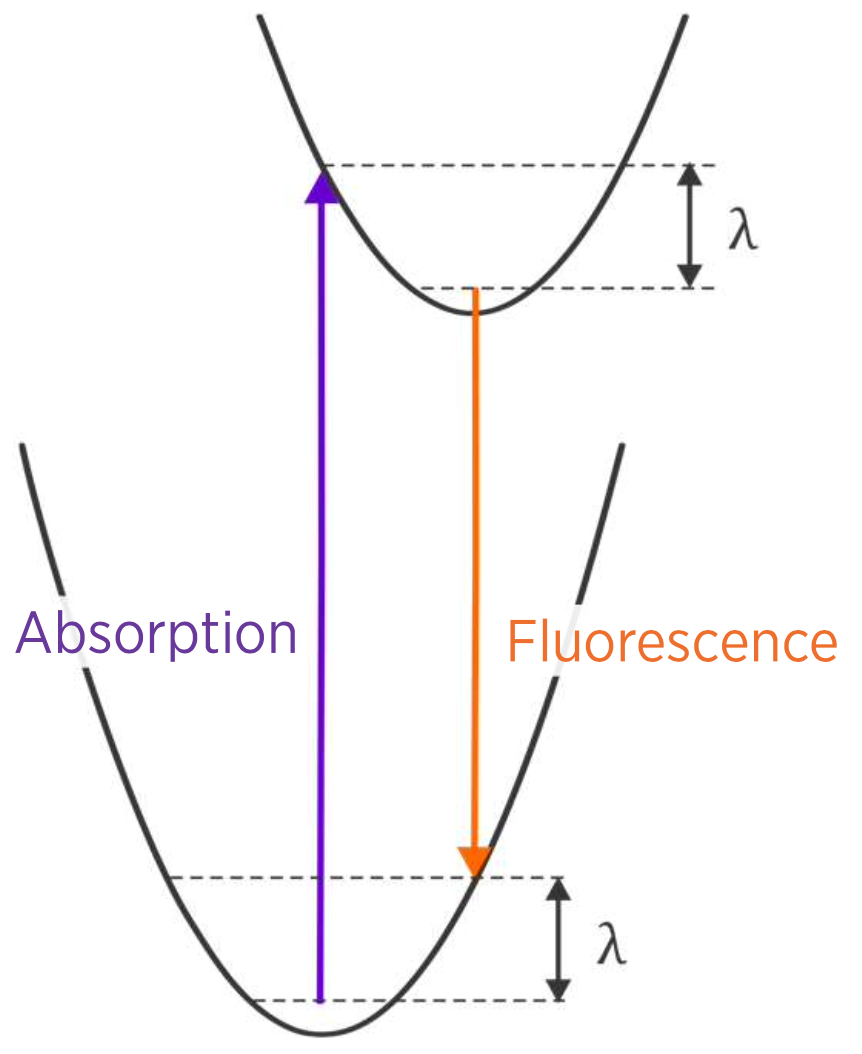
\includegraphics[width=0.6\linewidth]{reorgEa.png}
            \caption{Reorganization energy.}
            \label{fig:reorgEa}
        \end{subfigure}
        \begin{subfigure}[b]{0.35\linewidth}
            \centering
            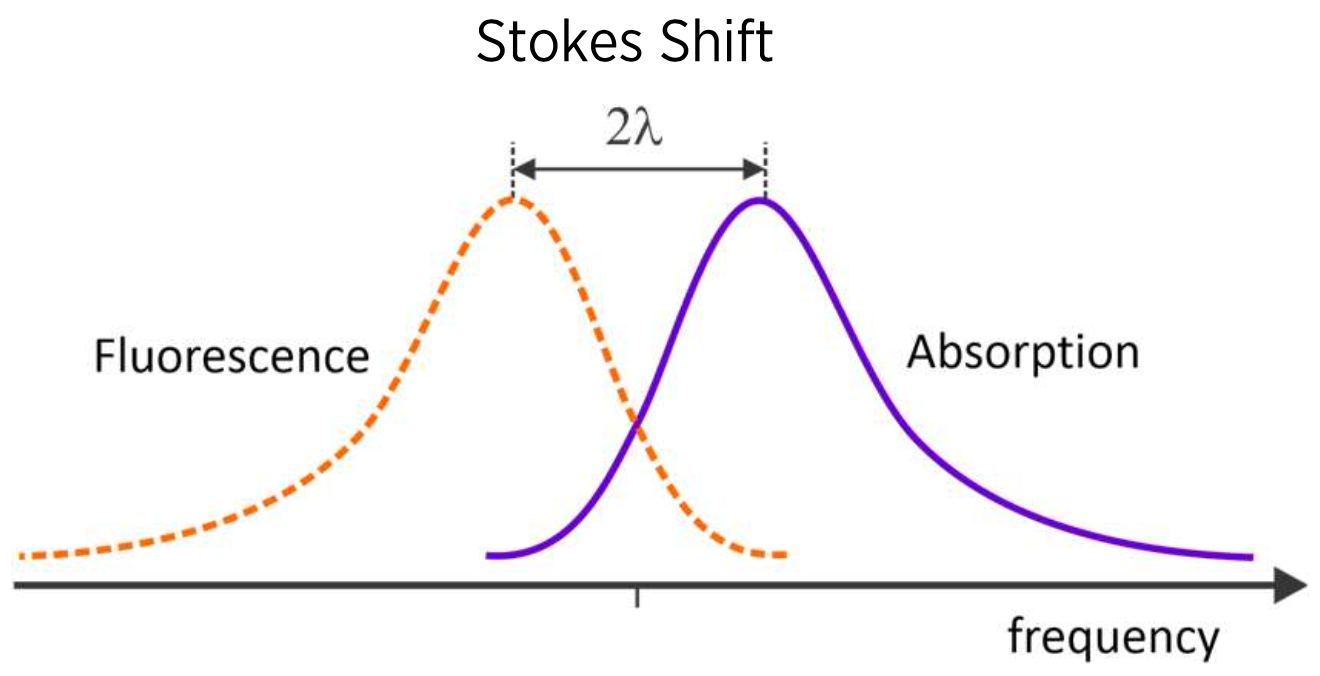
\includegraphics[width=0.95\linewidth]{reorgEb.png}
            \caption{Stokes shift.}
            \label{fig:reorgEb}
        \end{subfigure}
        \caption{Quantifying photophysical reorganization.}
        \label{fig:reorgE}
    \end{figure}
    \begin{itemize}
        \item Per the above, some energy is dissipated in both the ground and excited states. The amount dissipated in both is (roughly??) the same and is denoted by $\lambda$.
        \item The overall energy shift is known as the \textbf{Stokes shift} and is the sum of the two reorganizational energies.
    \end{itemize}
    \item \textbf{Stokes shift}: The difference in energy absorbed vs. energy fluoresced. \emph{Denoted by} $\bm{2\lambda}$.
    \item Other non-radiative intramolecular electronic relaxation process.
    \item Internal conversion.
    \begin{figure}[h!]
        \centering
        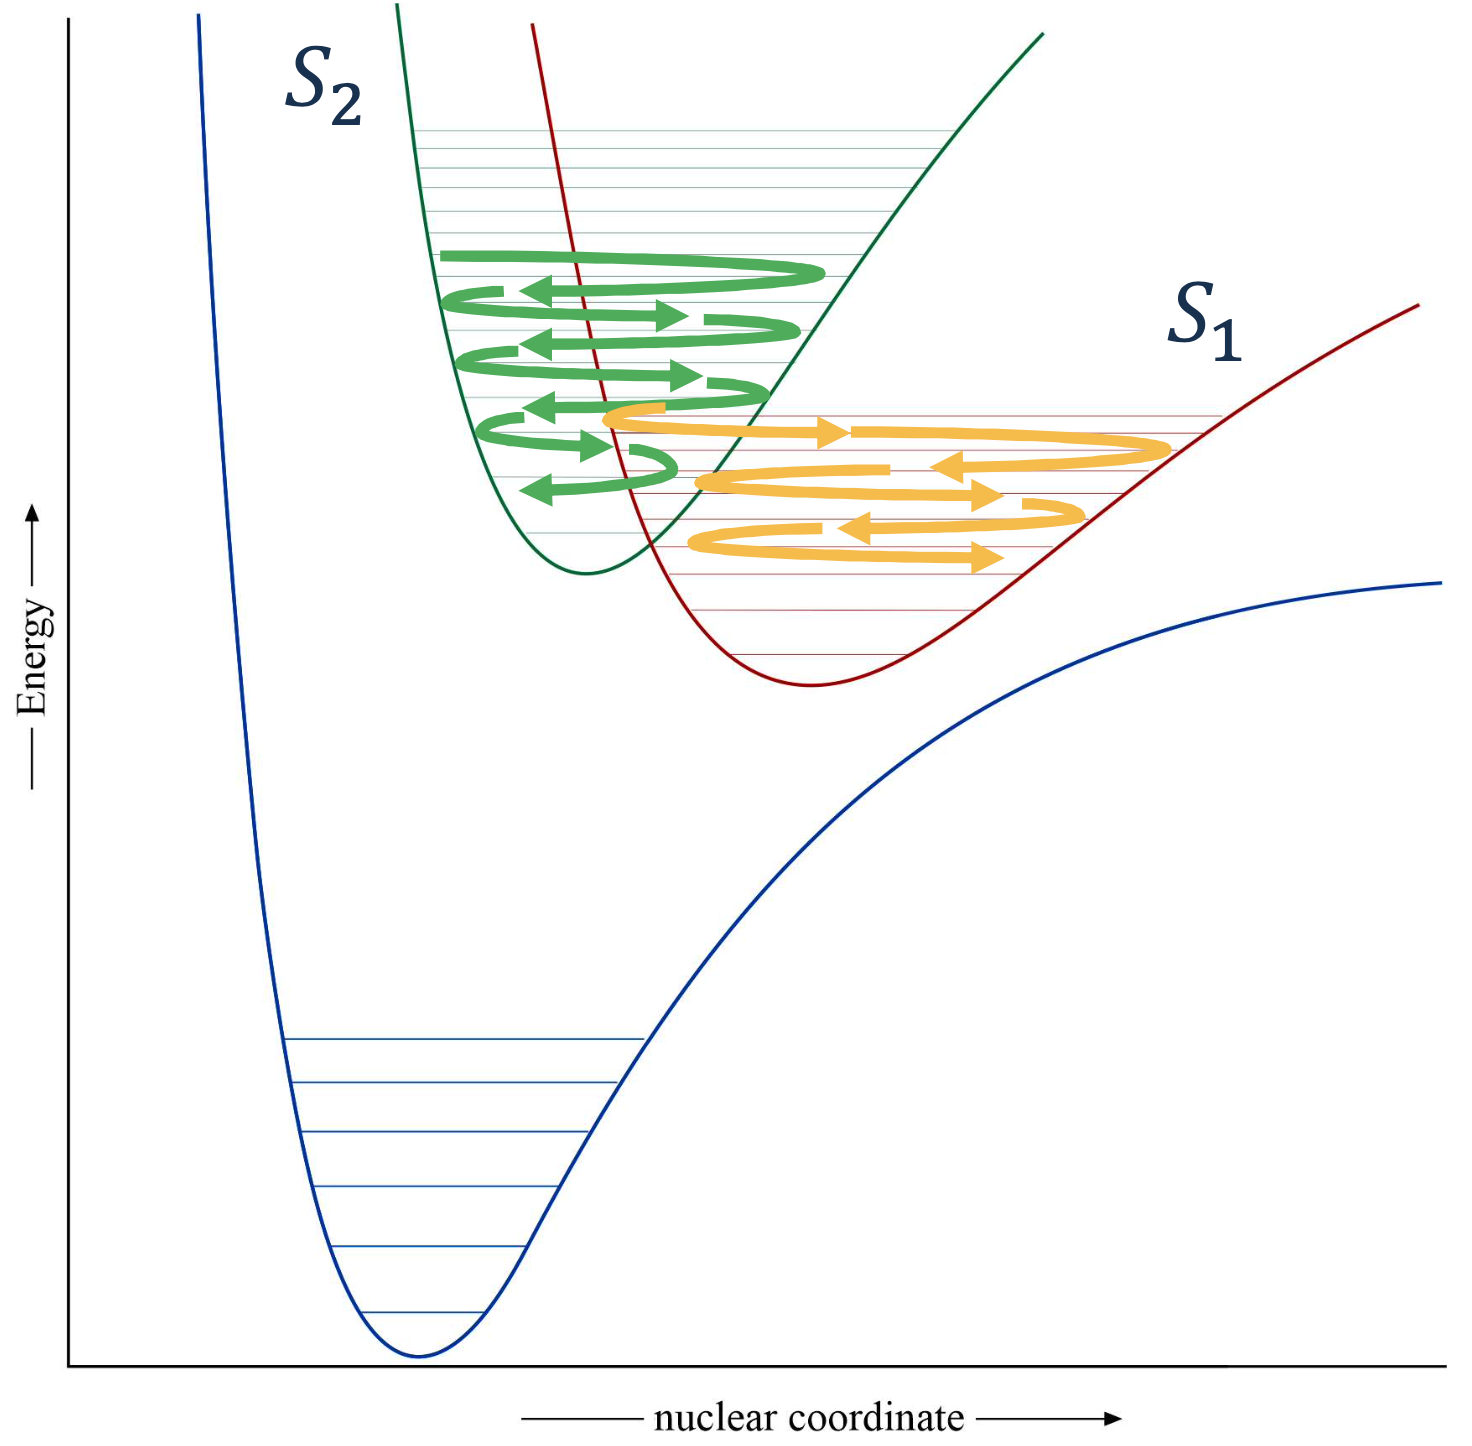
\includegraphics[width=0.3\linewidth]{internalConversion.png}
        \caption{Internal conversion.}
        \label{fig:internalConversion}
    \end{figure}
    \begin{itemize}
        \item Essentially, exchange between higher lying excited singlet states can be very efficient.
        \item We obey the \textbf{energy gap law}.
    \end{itemize}
    \item \textbf{Energy gap law}: The non-radiative relaxation rate scales exponentially in the energy gap between the initial and final states. \emph{Given by}
    \begin{equation*}
        k_\text{nr} \propto \exp(-\Delta E)
    \end{equation*}
    \item Intersystem crossing.
    \begin{itemize}
        \item Non-radiative singlet to triplet energy transfer.
        \item We have to consider what happens when we change the spin angular momentum. Because this takes energy, this is quite improbable unless we have something like spin-orbit coupling present.
        \item Nominally forbidden in closed shell molecules. Hence, it is slow.
        \begin{itemize}
            \item $ms$ in closed shell organics.
            \item $ps$-$ns$ in metal coordination compounds via SOC, MLCT.
        \end{itemize}
    \end{itemize}
    \item \textbf{Phosphorescence}: Luminescence from triplet states.
    \begin{itemize}
        \item Occurs on a very slow microsecond to millisecond time scale.
    \end{itemize}
    \item Intermolecular processes.
    \begin{figure}[h!]
        \centering
        \begin{subfigure}[b]{0.24\linewidth}
            \centering
            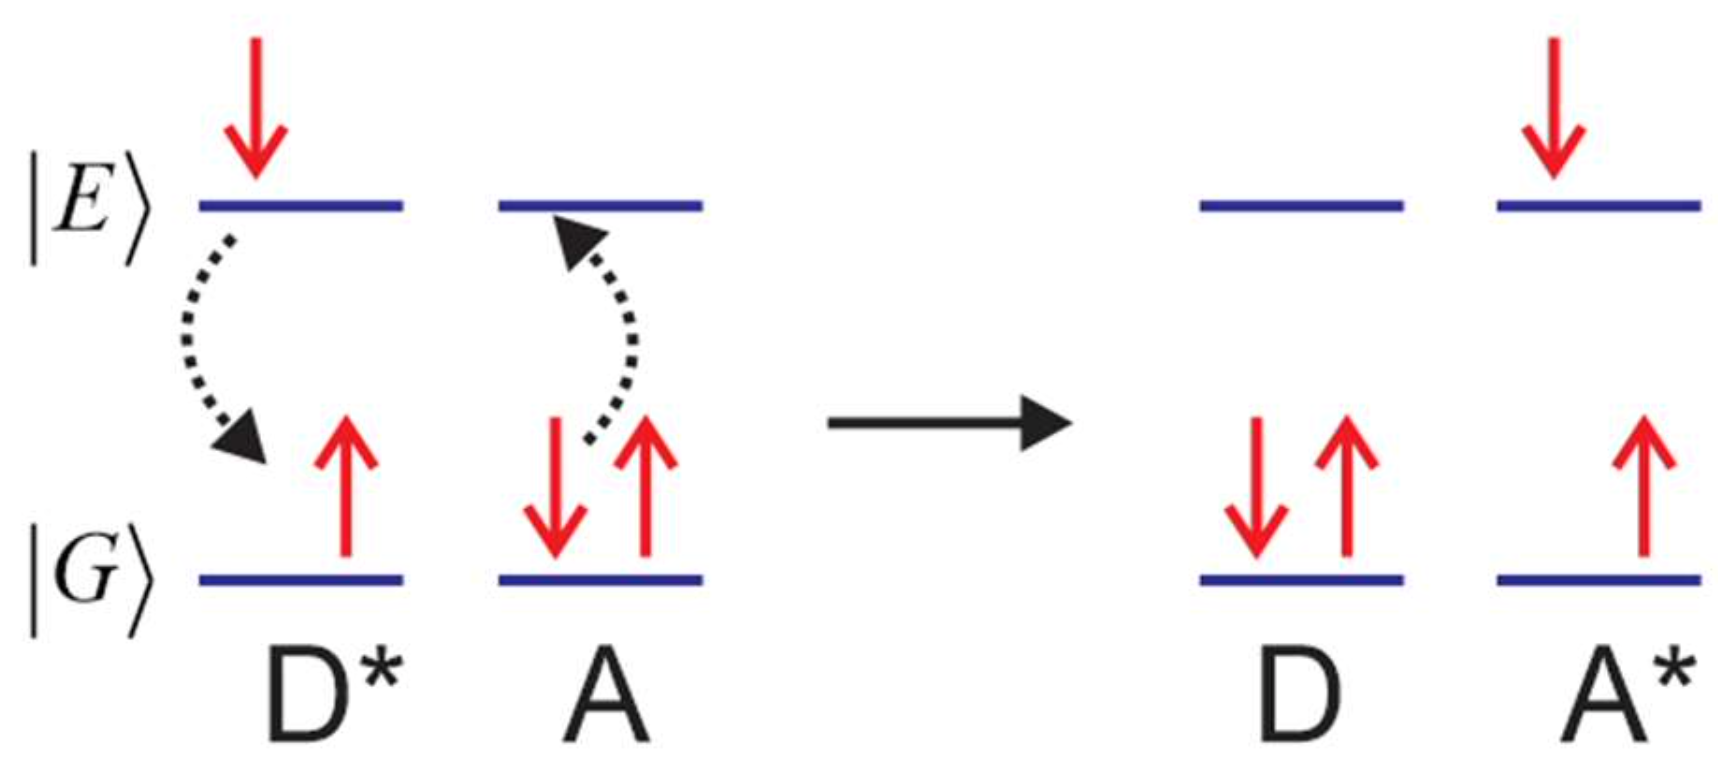
\includegraphics[width=0.8\linewidth]{interRelaxa.png}
            \caption{Forster ET.}
            \label{fig:interRelaxa}
        \end{subfigure}
        \begin{subfigure}[b]{0.24\linewidth}
            \centering
            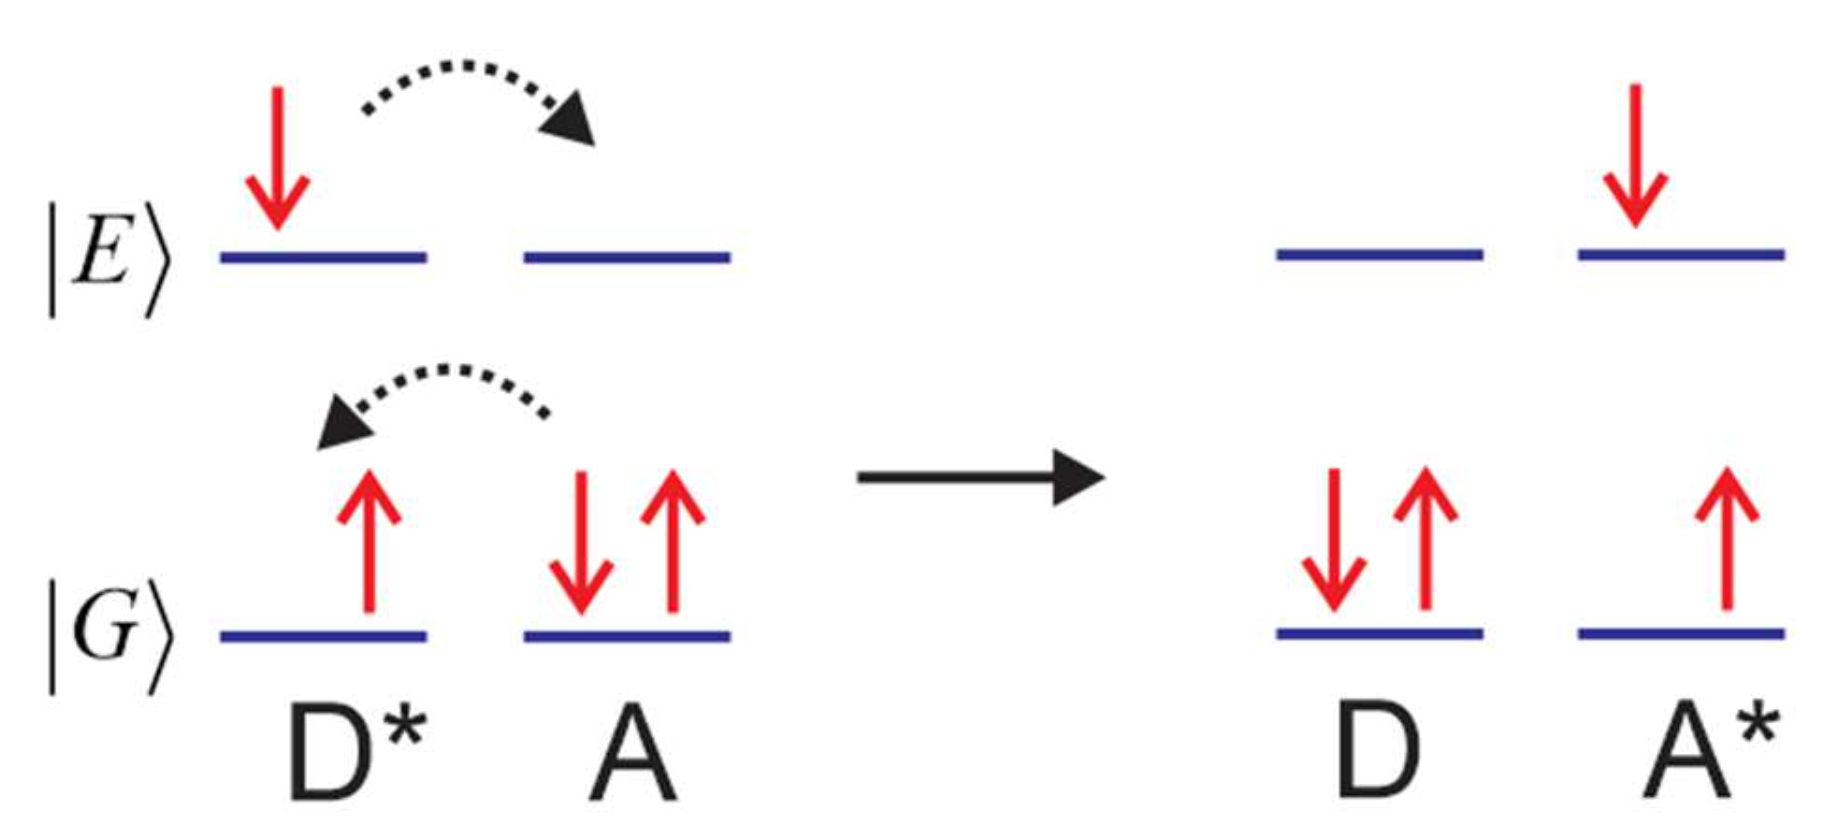
\includegraphics[width=0.8\linewidth]{interRelaxb.png}
            \caption{Dexter ET.}
            \label{fig:interRelaxb}
        \end{subfigure}
        \begin{subfigure}[b]{0.24\linewidth}
            \centering
            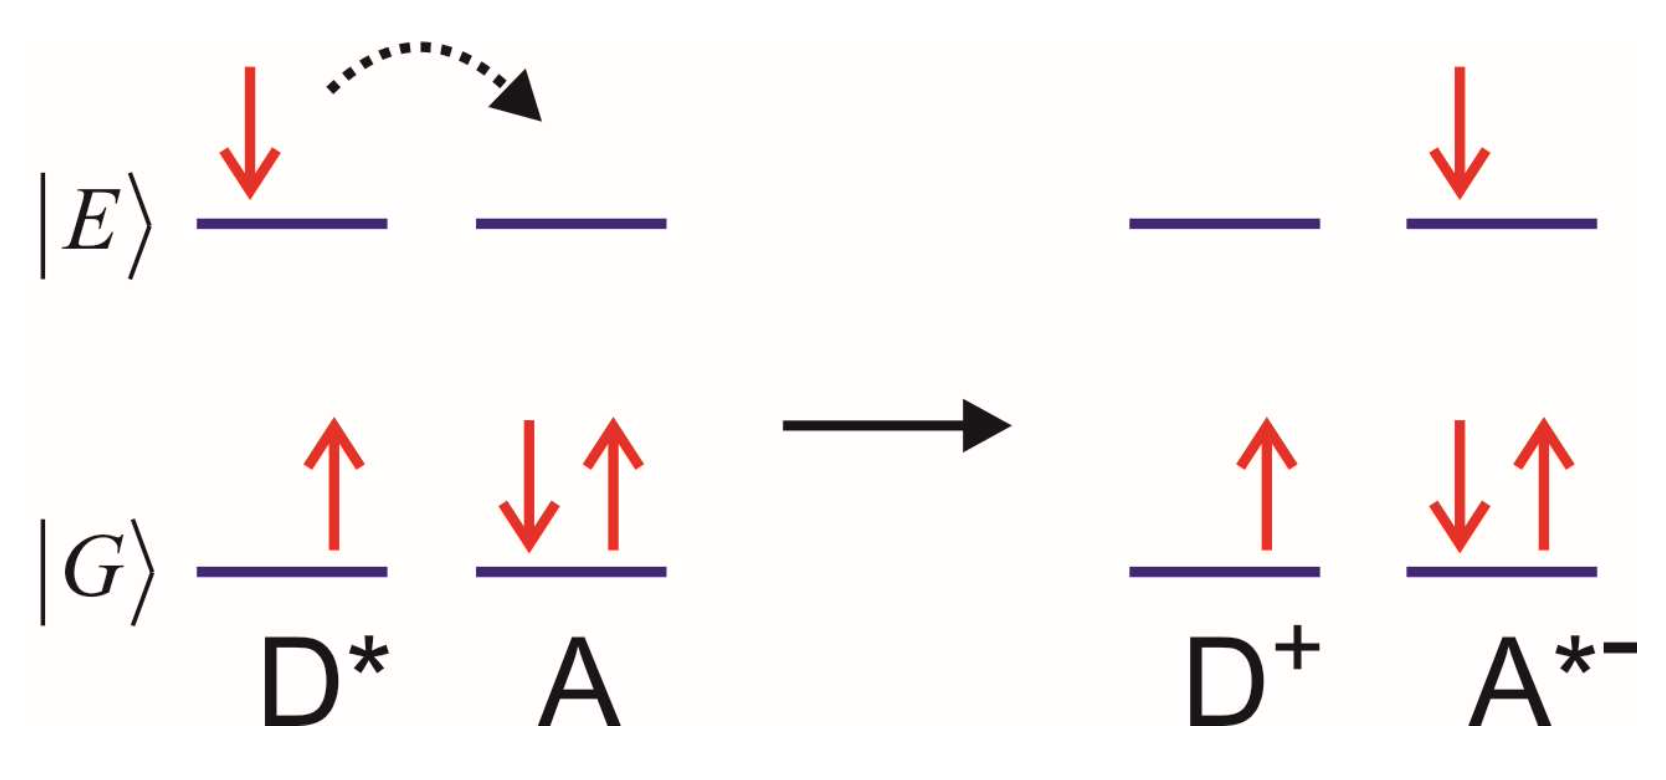
\includegraphics[width=0.8\linewidth]{interRelaxc.png}
            \caption{MLCT.}
            \label{fig:interRelaxc}
        \end{subfigure}
        \begin{subfigure}[b]{0.24\linewidth}
            \centering
            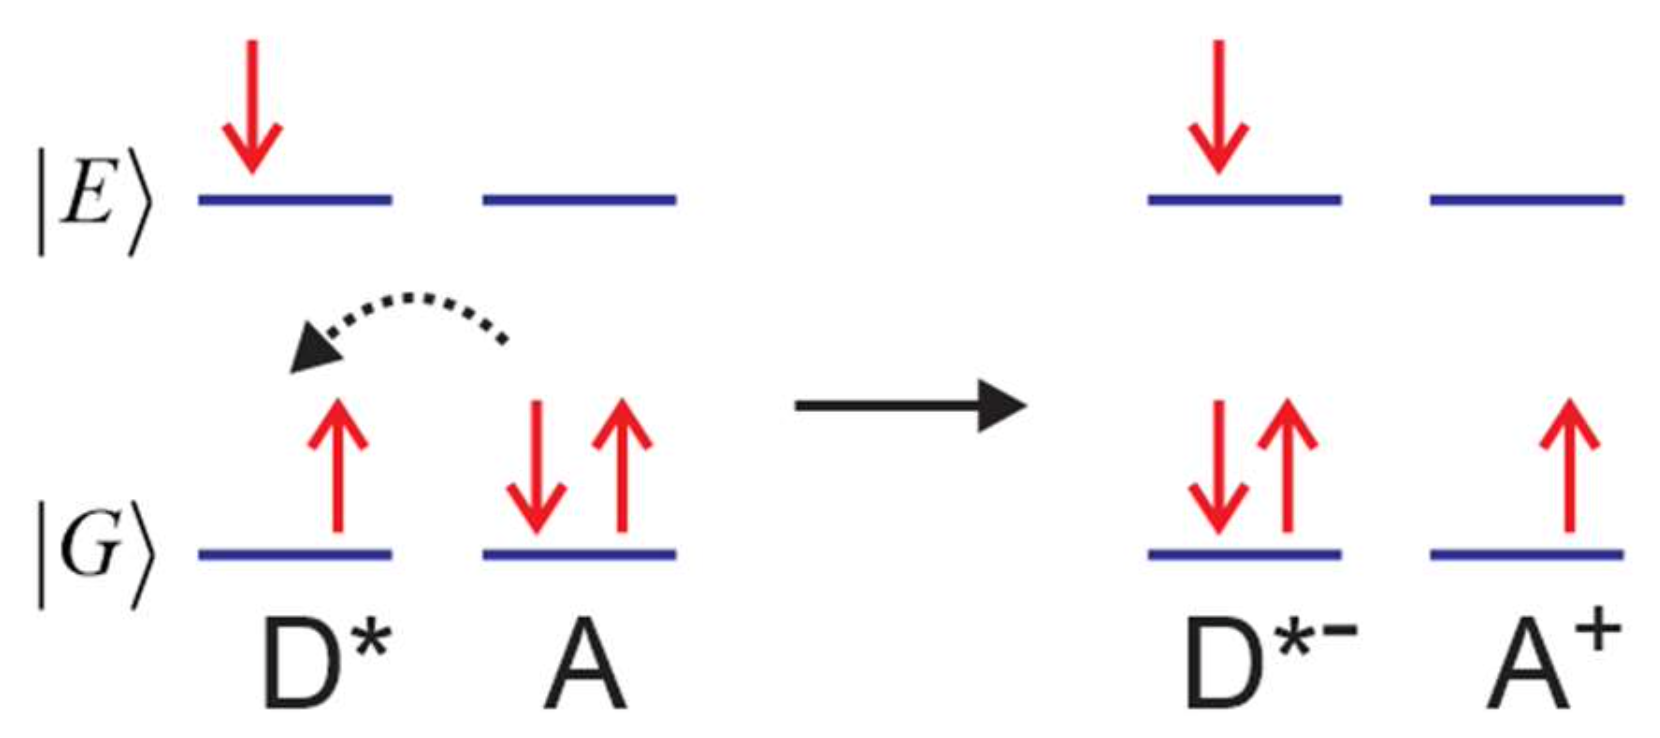
\includegraphics[width=0.8\linewidth]{interRelaxd.png}
            \caption{LMCT.}
            \label{fig:interRelaxd}
        \end{subfigure}
        \caption{Intermolecular relaxation mechanisms.}
        \label{fig:interRelax}
    \end{figure}
    \begin{itemize}
        \item Forster energy transfer (through space), aka, electronic resonance energy transfer.
        \begin{itemize}
            \item Two dipoles couple, and one drives the other.
        \end{itemize}
        \item Dexter energy transfer.
        \begin{itemize}
            \item Wavefunction overlap and electrons move.
        \end{itemize}
        \item MLCT (electron transfer).
        \begin{itemize}
            \item Donor gives a high energy electron to an acceptor.
        \end{itemize}
        \item LMCT (hole transfer).
        \begin{itemize}
            \item Donor gives a hole to the acceptor.
            \item Electronic excitation brings electron density to the metal center.
        \end{itemize}
    \end{itemize}
    \item Triplet quenching by oxygen.
    \begin{figure}[h!]
        \centering
        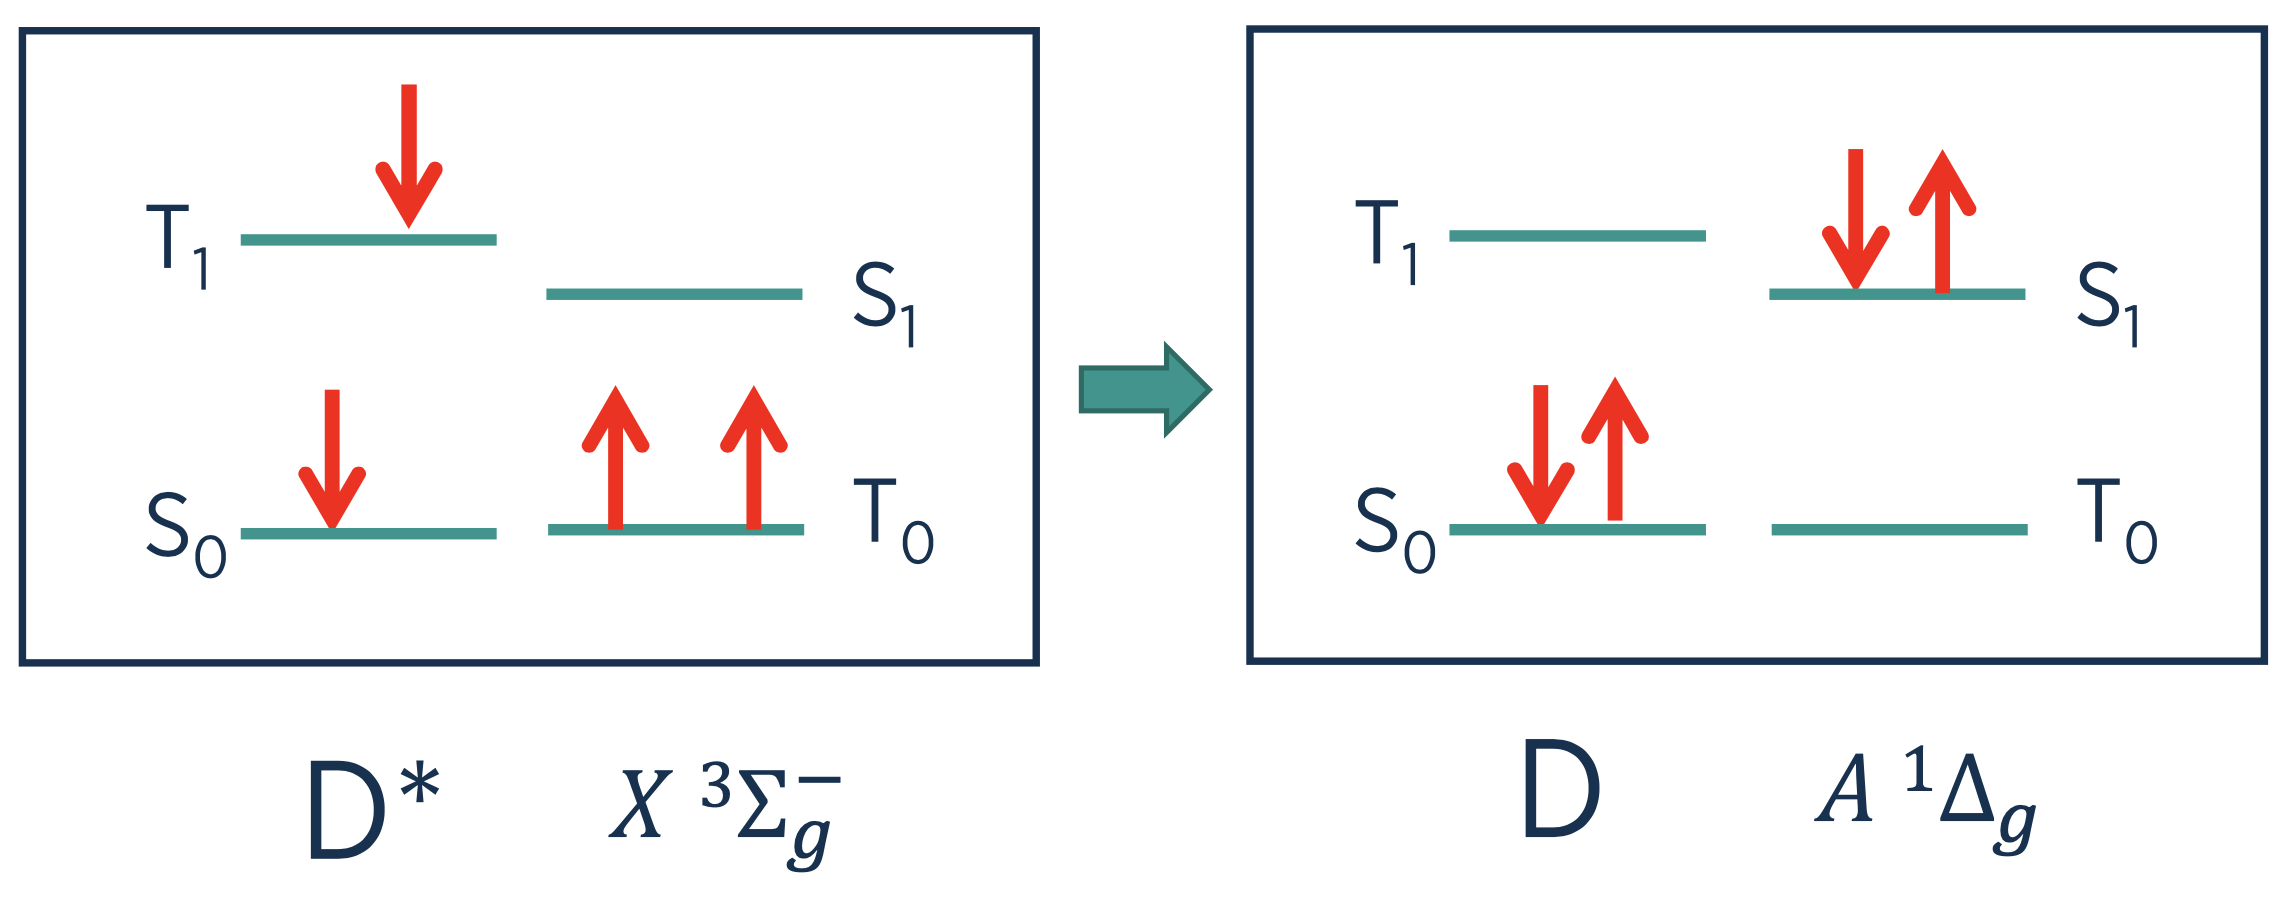
\includegraphics[width=0.4\linewidth]{O2TripQuench.png}
        \caption{Triplet quenching by oxygen.}
        \label{fig:O2TripQuench}
    \end{figure}
    \begin{itemize}
        \item Oxygen is a rare ground-state triplet compound.
        \item Thus, it can easily transfer electron density to other excited triplets, quenching them.
        \item Rate is partially determined by the proximity of oxygen to whatever it's quenching.
    \end{itemize}
    \item Photochemistry summary.
    \begin{itemize}
        \item Light provides energy to surmount activation barriers (relevant to atmospheric chemistry, photosynthesis).
        \item Photodissociation (relevant to bond cleavage, ligand release, photoacids, photoionization, and radicals).
        \item Electron transfer and proton-coupled electron transfer.
        \item Photoisomerization (see below).
    \end{itemize}
    \item Photoisomerization.
    \begin{figure}[h!]
        \centering
        \begin{subfigure}[b]{0.5\linewidth}
            \centering
            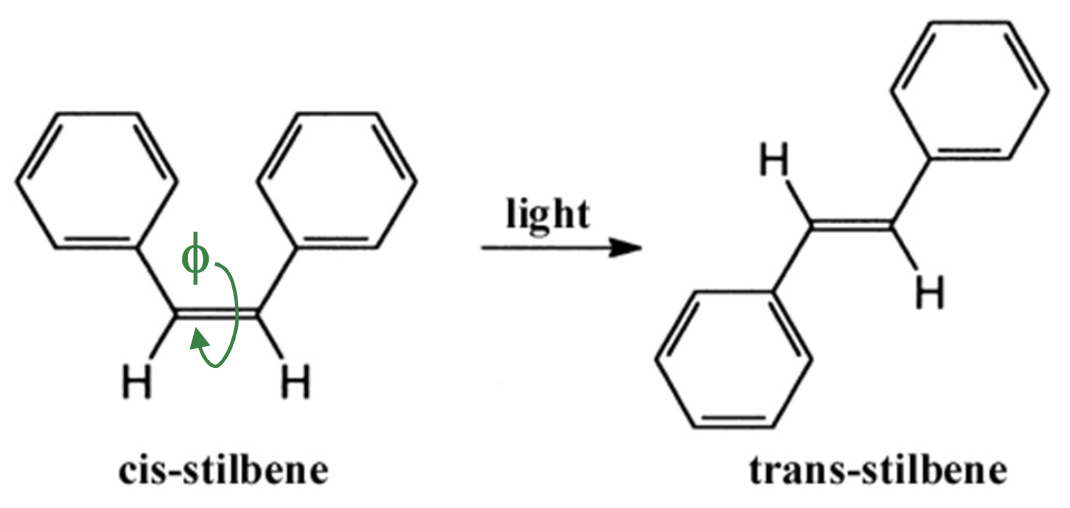
\includegraphics[width=0.8\linewidth]{photoisomerizationa.png}
            \caption{Example reaction.}
            \label{fig:photoisomerizationa}
        \end{subfigure}
        \begin{subfigure}[b]{0.3\linewidth}
            \centering
            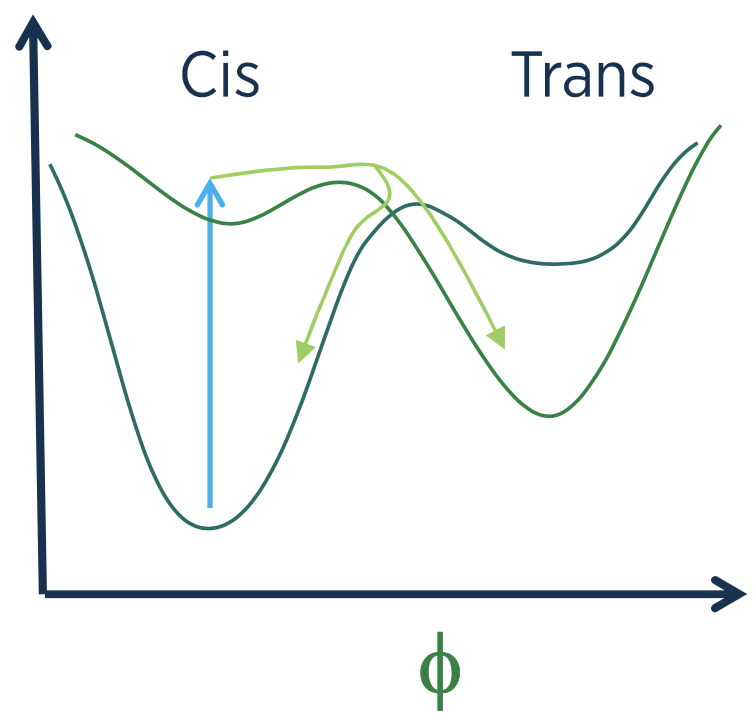
\includegraphics[width=0.8\linewidth]{photoisomerizationb.png}
            \caption{Mechanism.}
            \label{fig:photoisomerizationb}
        \end{subfigure}
        \caption{Photoisomerization.}
        \label{fig:photoisomerization}
    \end{figure}
    \begin{itemize}
        \item Stilbene possesses \emph{cis}/\emph{trans} photoisomerization.
    \end{itemize}
    \item Quantities in fluorescence spectroscopy.
    \item \textbf{Fluorescence quantum yield}: The probability that an absorbed photon led to emission of a photon via fluorescence. \emph{Denoted by} $\bm{\Phi}$. \emph{Given by}
    \begin{equation*}
        \Phi = \frac{\text{\# of fluorescence photons emitted}}{\text{\# of input photons absorbed}}
        = \frac{k_\text{rad}}{k_\text{rad}+k_\text{nr}}
    \end{equation*}
    \begin{itemize}
        \item Tells you how good of a fluorophore your molecule is, i.e., how good it is at absorbing light and turning it back into fluorescence.
    \end{itemize}
    \item $\bm{k_\textbf{f}}$: The rate constant for fluorescence emission. \emph{Given by}
    \begin{equation*}
        k_\text{f} = k_\text{rad}+k_\text{nr}
    \end{equation*}
    \item \textbf{Fluorescence lifetime}: The time constant relating to the rate of fluorescence emission. \emph{Denoted by} $\bm{\tau}$. \emph{Given by}
    \begin{equation*}
        \tau = \frac{1}{k_\text{f}}
    \end{equation*}
    \item The underlying theory behind the fluorescence lifetime.
    \begin{itemize}
        \item The measured fluorescence intensity $I(t)$ is proportional to the number of excited states, i.e.,
        \begin{equation*}
            I(t) \propto \ce{A^*}(t)
        \end{equation*}
        \item The rate law for fluorescence decay is
        \begin{align*}
            \dv{\ce{A^*}}{t} &= -k_\text{f}\ce{A^*}\\
            I(t) &= I(0)\exp(-k_\text{f}t)
        \end{align*}
    \end{itemize}
    \item Implication: We can use fluorescence to probe non-radiative processes.
    \item Example: Quenching experiments.
    \begin{itemize}
        \item Object of study: Short-range interactions that lead to rapid non-radiative relaxation.
        \item Background: The fluorescence lifetime in the absence of quencher is $\tau_0=k_0^{-1}$. The quencher results in an additional route for non-radiative relaxation.
        \begin{itemize}
            \item Implication: The fluorescence lifetime $\tau$ decreases: $\tau<\tau_0$.
            \item If $[\ce{Q}]$ denotes the concentration of the quencher and $k_q$ denotes the rate constant associated with quenching by the quencher, then we have
            \begin{align*}
                -\dv{\ce{A^*}}{t} &= k_0\ce{A^*}+k_q\ce{A^*}[\ce{Q}]\\
                &= (k_0+k_q[\ce{Q}])\ce{A^*}
            \end{align*}
            so that
            \begin{equation*}
                \frac{1}{\tau} = k_0+k_q[\ce{Q}]
                = \frac{1}{\tau_0}+k_q[\ce{Q}]
            \end{equation*}
        \end{itemize}
        \item Analysis: Use a \textbf{Stern-Volmer plot}.
        \begin{itemize}
            \item Acquire fluorescence lifetime as a function of the quencher concentration using the last equation above.
            \item This gives us the rate constant $k_q$ as the slope and $1/\tau_0$ as the $y$-intercept.
        \end{itemize}
    \end{itemize}
    \item Quantum dots: Electrons in confinement.
    \begin{figure}[H]
        \centering
        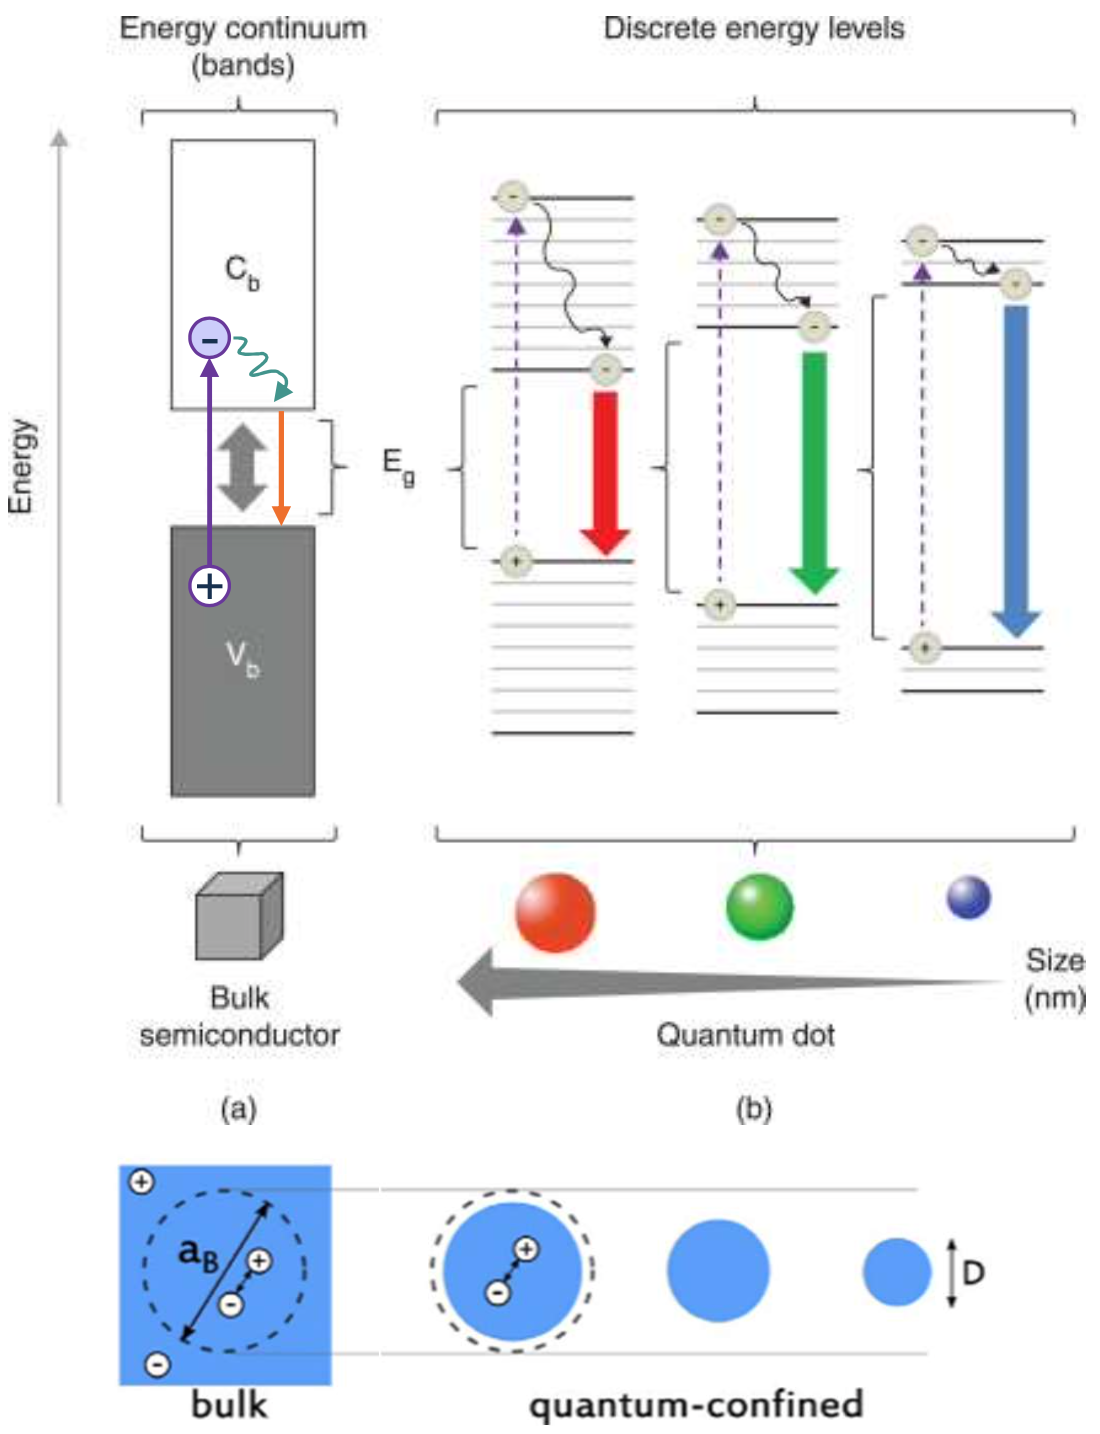
\includegraphics[width=0.4\linewidth]{QDotsConfinement.png}
        \caption{Quantum confinement effects in QDots.}
        \label{fig:QDotsConfinement}
    \end{figure}
    \begin{itemize}
        \item Nanomaterials: Size-dependent optical properties.
        \item The color changes from blue to red as the size of \ce{CdSe} nanodots grows from \SI{2}{\nano\meter} to \SI{8}{\nano\meter}.
        \item Why?
        \begin{itemize}
            \item In a bulk semiconductor, excitation creates an \textbf{exciton}.
            \item Excited electron and hole can diffuse.
            \item Dissipation of heat to lattice (via \textbf{phonons}).
            \item Emission of light at the bandgap $E_g$.
            \item The electron and hole attract coulombically, but there is a length scale in bulk; this is why size affects color.
        \end{itemize}
        \item Confinement: We confine the exciton to tiny sphere (like the particle in a box), but then only certain energy levels (corresponding to colors based on size) can be taken on.
        \item The Coulomb potential leads to hydrogen-like energies and wavefunctions.
    \end{itemize}
    \item \textbf{Exciton}: An electron-hole pair.
\end{itemize}




\end{document}